\documentclass[12pt]{article}
\usepackage[top=1in,bottom=1in,left=0.75in,right=0.75in,centering]{geometry}
\usepackage{fancyhdr}
\usepackage{epsfig}
\usepackage[pdfborder={0 0 0}]{hyperref}
\usepackage{palatino}
\usepackage{wrapfig}
\usepackage{lastpage}
\usepackage{color}
\usepackage{ifthen}
\usepackage[table]{xcolor}
\usepackage{graphicx,type1cm,eso-pic,color}
\usepackage{hyperref}
\usepackage{amsmath}
\usepackage{wasysym}
\usepackage{amsfonts}

\def\course{CS 3120: Discrete Math and Theory II}
\def\homework{Set Cardinality}
\def\semester{Fall 2024}

\newboolean{solution}
\setboolean{solution}{false}

% add watermark if it's a solution exam
% see http://jeanmartina.blogspot.com/2008/07/latex-goodie-how-to-watermark-things-in.html
\makeatletter
\AddToShipoutPicture{%
\setlength{\@tempdimb}{.5\paperwidth}%
\setlength{\@tempdimc}{.5\paperheight}%
\setlength{\unitlength}{1pt}%
\put(\strip@pt\@tempdimb,\strip@pt\@tempdimc){%
\ifthenelse{\boolean{solution}}{
\makebox(0,0){\rotatebox{45}{\textcolor[gray]{0.95}%
{\fontsize{5cm}{3cm}\selectfont{\textsf{Solution}}}}}%
}{}
}}
\makeatother

\pagestyle{fancy}

\fancyhf{}
\lhead{\course}
\chead{Page \thepage\ of \pageref{LastPage}}
\rhead{\semester}
%\cfoot{\Large (the bubble footer is automatically inserted into this space)}

\setlength{\headheight}{14.5pt}

\newenvironment{itemlist}{
\begin{itemize}
\setlength{\itemsep}{0pt}
\setlength{\parskip}{0pt}}
{\end{itemize}}

\newenvironment{numlist}{
\begin{enumerate}
\setlength{\itemsep}{0pt}
\setlength{\parskip}{0pt}}
{\end{enumerate}}

\newcounter{pagenum}
\setcounter{pagenum}{1}
\newcommand{\pageheader}[1]{
\clearpage\vspace*{-0.4in}\noindent{\large\bf{Page \arabic{pagenum}: {#1}}}
\addtocounter{pagenum}{1}
\cfoot{}
}

\newcounter{quesnum}
\setcounter{quesnum}{1}
\newcommand{\question}[2][??]{
\begin{list}{\labelitemi}{\leftmargin=2em}
\item [\arabic{quesnum}.] {} {#2}
\end{list}
\addtocounter{quesnum}{1}
}


\definecolor{red}{rgb}{1.0,0.0,0.0}
\newcommand{\answer}[2][??]{
\ifthenelse{\boolean{solution}}{
\color{red} #2 \color{black}}
{\vspace*{#1}}
}

\definecolor{blue}{rgb}{0.0,0.0,1.0}

\begin{document}

\section*{\homework}


\question[3]{
For each of the following claims, state whether it is true or false and then prove your assertion.
}

\begin{itemize}
	\item All finite sets have an \emph{injection} to $\mathbb{N}$
	\item All finite sets have a \emph{surjection} to $\mathbb{N}$
	\item If $A$ is a countably infinite set (i.e., $|A|=|\mathbb{N}|$) and $B$ is a also a countably infinite set (i.e., $|B| = |\mathbb{N}|$), then $A \cup B$ is also countable.
	\item If $A$ is countably infinite and $B$ is uncountably infinite, then $A \cup B$ is countable.
	\item If $A$ is countably infinite and $B$ is uncountably infinite, then $A \cap B$ is countable.
\end{itemize}

\vspace{12pt}



\question[3]{
Consider a square grid with length and width $n$. The bottom left corner is considered position $(0,0)$ and the upper right corner is position $(n,n)$ \emph{(*Note that the first item in the tuple is the square along the horizontal axis and the second element is the index along the vertical axis)}. You can see an example grid below.\\
\\
Our goal is to find all the unique ways a robot starting at cell $(0,0)$ can reach cell $(n,n)$ by only moving up, down, left, right on the grid on each move. We would like you to do two things:

\begin{enumerate}
	\item In your own words, argue why the given set (the set of possible paths to the goal) is infinite (as opposed to finite).
	\item Show that the set of unique paths the robot can take to reach position $(n,n)$ is \emph{countably infinite}. \emph{Hint: Try showing that a superset of this one is countably infinite}.
\end{enumerate}
}

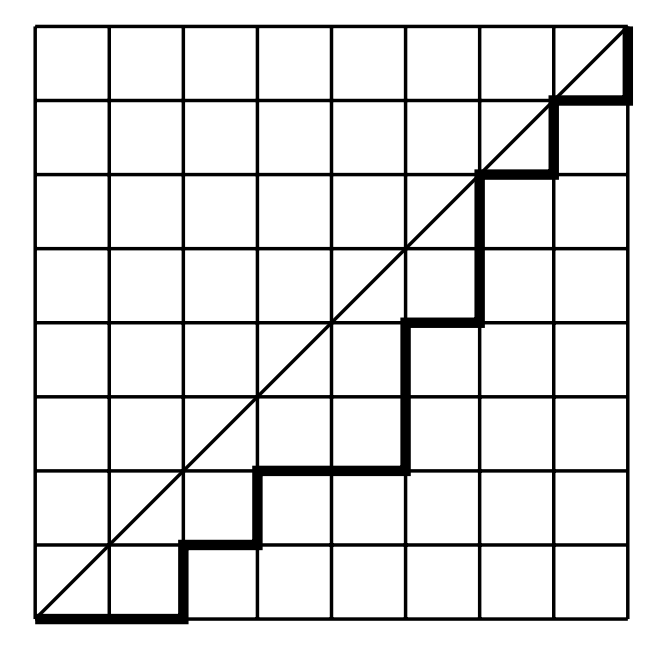
\includegraphics[scale=0.4]{img/lattice}

\vspace{12pt}

\question[3]{
Use a proof by diagonalization to show that the following set is uncountable:\\
\\
$F= \mathcal{P}(\mathbb{N}) $
\\
\\
In other words, prove that the power set of the natural numbers (the set of all subsets of the natural numbers) is uncountable.
}

\vspace{12pt}



\end{document}
